\section{Iris Recognition}
\label{sec:Iris_Recognition_Research}
Modern iris recognition started in with an article by \cite{Daugman1993} discussing the security of using iris for recognition. An outline of how to do recognition was also laid out with the introduction of using  2D Gabor Waveletts to extract features of the complex pattern that can be found in an iris. This methodology has since been the basis for most iris recognition. It was also the foundation for IrisCode which is a commercially developed iris recognition algorithm by John Daugman. In 2016 a handbook for iris recognition by \cite{Bowyer2016b} was published giving an outline of the whole process of iris recognition. In general Near Infra-Red (NIR) images of an iris are used but other type of images can also be used.  \cite{Khan2017a} show how to use Daugmans methodology on iris images taken with a smartphone in visible light. They use Daugmans Integro-differential operator to localise the bounds of the iris. Then they suppress the eyelids the eyelids which often cover parts of the iris by using an approach inspired by Masek. Afterwards the image is normalised by using the homogeneous rubber sheet model by Daugman. Then eyelashes are removed from the image and feature extraction is done by using 2D Gabor Waveletts. This approach to extract features in one way or another can be seen in multiple state of the art iris recognition systems and research papers e.g \citep{Luhadiya2017a,Uka2017a,Kuehlkamp2016a}, \cite{Kuehlkamp2016a}. After the features have been extracted they are compared/categorised. Traditionally a "1-to-N search" has been done. Here the Hamming distance of features of the scanned iris are compared to the whole database and it is classified with the iris that has the least distance. \cite{Kuehlkamp2016a} have suggested using a "1-to-first search" instead to improve the speed of the search. Here a threshold is chosen and as soon as a match has been found below the threshold it will stop the search. Other approaches to the categorisation have been proposed using machine learning. \cite{Khan2017a} proposed using Support Vector Machines (SVM), K-Nearest-Neighbours(KNN) and Linear Discriminant Analysis (LDA) with respective test accuracies of 97\%, 95.1\%, 94.28\%. \cite{Zhao2017b} proposed using deep learning to classify. They claim that research in neural networks with iris recognition is still very new and not much has been done. But some of the work that has been done have used Convolutional Neural Networks (CNN) and a Deep Belief Network (DBN). They claim that the problem with traditional networks are that they are very database specific on not very generalisable. \cite{Zhao2017b} created a Fully Convolutional Network (FCN) using a loss function they created specifically for iris networks called Extended Triplet Loss (ETL). They claim this network is more generalisable than the previous networks. \cite{RifaeeMustafaandAbdallahMohammadandOkosh2017a} gives an outline of commercially free databases often used in research.\autoref{fig:Iris_database_1} and \autoref{fig:Iris_database_2} show the different contents of the databases. 

\begin{figure}
\centering
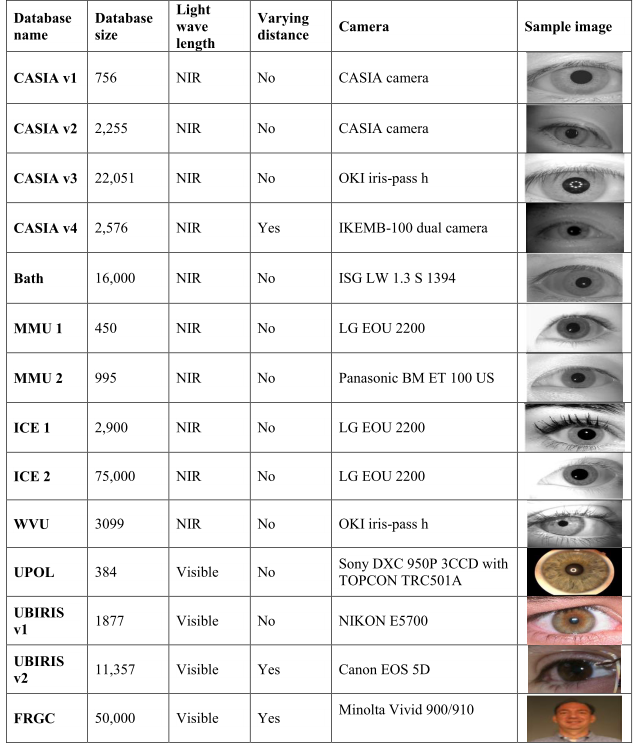
\includegraphics[width=\textwidth]{figures/Iris_Database_tabel_1.png} 
\caption{A table depicting the contents of free iris image databases.}
\label{fig:Iris_database_1}
\end{figure}

\begin{figure}
\centering
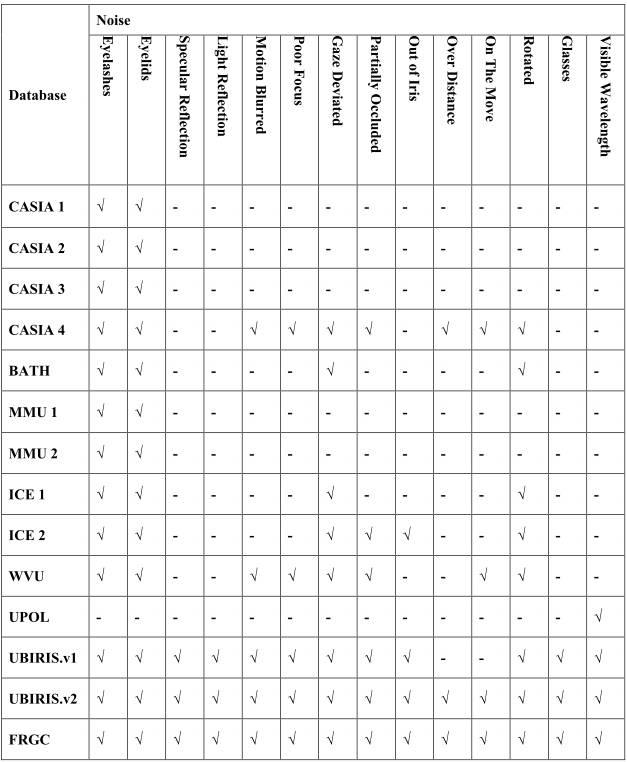
\includegraphics[width=\textwidth]{figures/Iris_Database_tabel_2.png} 
\caption{A table depicting the noise present in the databases}
\label{fig:Iris_database_2}
\end{figure}

